
% neue Folie
\newpage
\slidetitle{}
\section{Lindenmayer-Systeme \\}

\begin{itemize}
	\item Von Aristid Lindenmayer 1968 entwickelte Erweiterung von Ersetzungssystemen \\
	
	\item Weitere Ergänzungen durch Prusinkiewicz und Lindenmayer in 1990\\
	
	\item Funktionsweise basiert auf der Ersetzung von Zeichen in Zeichenketten \\
	
	\item Grafische Interpretation der Resultate ergibt Modelldaten
	
\end{itemize}





\newpage
\slidetitle{2. L-Systeme - D0L-Systeme}

\subsection{D0L-Systeme\\ }
\newtheorem{defD0LSystem}{Definition D0L-System:}[subsection]
\begin{defD0LSystem}
	Ein deterministisches, kontextfreies L-System (D0L-System) ist ein Tupel G = $(V, P, \omega)$ mit:
	
	\begin{description}
		\item[\boldmath$V:$ ] Ein nichtleeres, endliches Alphabet\\
		
		\item[\boldmath$P:$ ] Eine Menge von Produktionsregeln in der Form $P: a \rightarrow b$ mit $a \in V$ und $b \in V^*$ \\
		
		\item[\boldmath$\omega \in V^+ :$ ]  Das Axiom, Startwort des L-Systems		
	\end{description}
\end{defD0LSystem}





\newpage

\paragraph{Verwendete Begriffe:\\}

\begin{description}
	\item[\textbf{Deterministisch:}] Es existiert genau eine Produktionsregel für jedes der Symbole in $V$ \\
	
	\item[\textbf{Kontextfrei:}] Ersetzung findet unabhängig von umgebenden Symbolen statt \\
	
	\item[\textbf{Ableitung:}] Gleichzeitige Ersetzung aller Symbole eines Wortes anhand der Produktionsregeln
	
\end{description}





\newpage
\slidetitle{2. L-Systeme - D0L-Systeme}

\paragraph{Beispiel: Simulation des Wachstums der Blaualgen-Gattung \glqq Anabaena\grqq{} \\}

  
\begin{description}
	\item[\boldmath$V$]  besteht aus den Symbolen \boldmath$\{a_l, a_r, b_l, b_r\}$
	\begin{description}
		\item[\boldmath$a$ und \boldmath$b$:] Größe und Teilungsbereitschaft einer Zelle\\
		\item[\boldmath$l$ und \boldmath$r$:] Zellenpolarität
	\end{description}
	\item[\boldmath$P$] besteht aus:
	\begin{description}
		\item[\boldmath$p_1 :$] $\begin{array}{ccc} a_r & \rightarrow & a_lb_r \end{array}$
		\item[\boldmath$p_2 :$] $\begin{array}{ccc} a_l &\rightarrow& b_la_r \end{array}$
		\item[\boldmath$p_3 :$] $\begin{array}{ccc} b_r &\rightarrow& a_r \end{array}$
		\item[\boldmath$p_4 :$] $\begin{array}{ccc} b_l &\rightarrow& a_l  \end{array}$
	\end{description}
\end{description}





\newpage

\begin{center}
	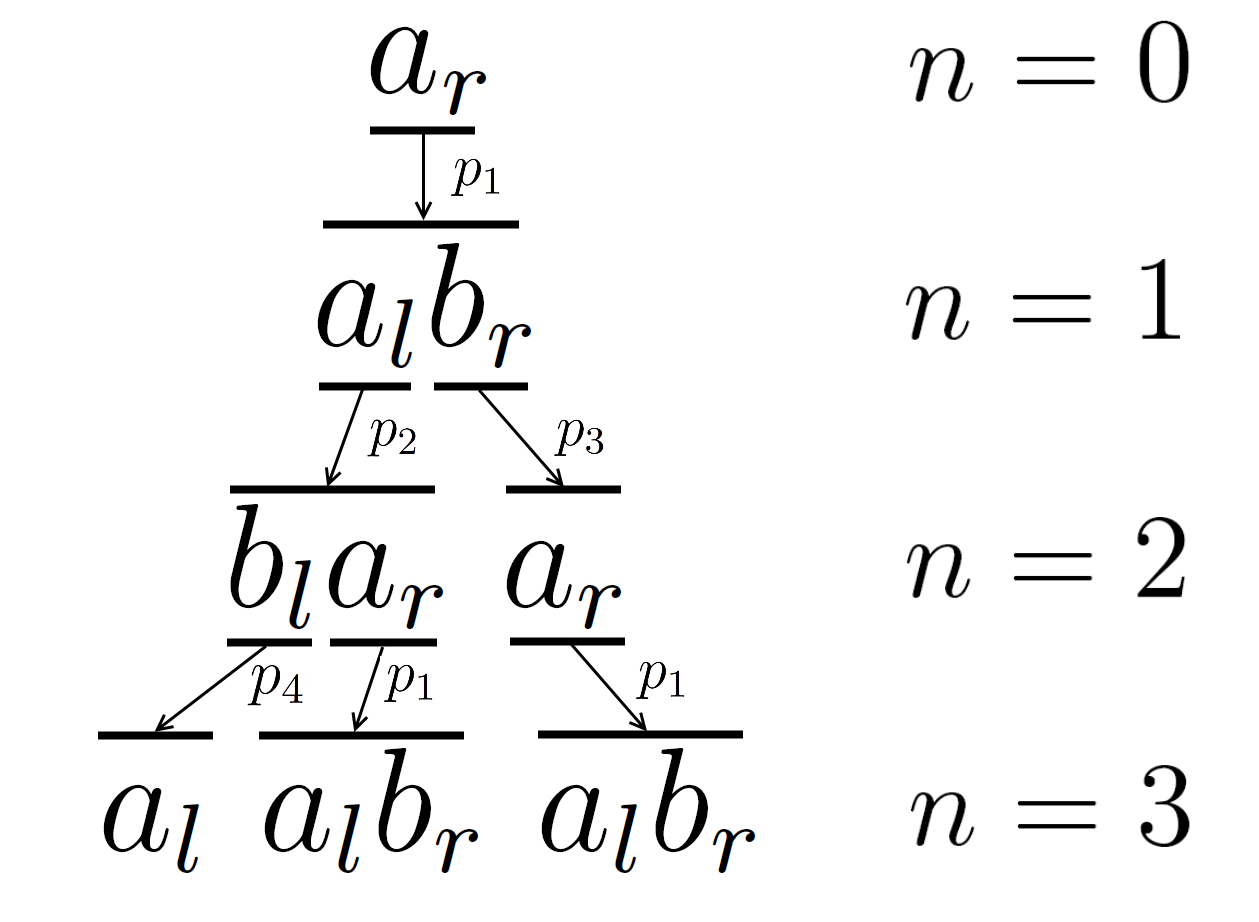
\includegraphics[height=1\textheight]{images/CH2_AnabaenaAbleitung.png}
\end{center}





\newpage
\slidetitle{2. L-Systeme - parametrische L-Systeme}
\subsection{Parametrische L-Systeme\\ }

\begin{itemize}
	\item Erweiterung der D0L-Systeme \\
	
	\item Verwendung von parametrischen Wörtern anstatt einfacher Symbole:
	\begin{description}
			\item[\boldmath$A(a_1, ..., a_n):$] Parametrisches Wort mit $A\in V$ und $a_1, ..., a_n \in \Sigma$\\
		
			\item[\boldmath$\Sigma:$] Menge formaler Parameter\\
	\end{description}
	
	\item Verwendung arithmetischer Ausdrücke im Nachfolger möglich
	%\begin{description}
		
	%	\item[\boldmath$E(\Sigma):$] Arithmetischer Ausdruck
	%\end{description}

\end{itemize}




\iffalse
\newpage
\paragraph{}
\newtheorem{defParametrischeLSysteme}{Parametrisches L-System:}[subsection]
\begin{defParametrischeLSysteme}
	Ein Parametrisches L-System ist ein Tupel G = $(V, \Sigma, P, \omega)$ mit:
	\begin{description}
		\item[\boldmath$V:$] Ein nichtleeres, endliches Alphabet\\
		
		\item[\boldmath$\Sigma:$] Eine Menge formaler Parameter\\
		
		\item[\boldmath$P:$] Eine Menge von Produktionsregeln $P : (V\times \Sigma^*) \rightarrow (V\times E(\Sigma)^*)^*$\\
		
		\item[\boldmath$\omega \in M^+$] mit $M =(V \times \mathbb{R}^*)$ -- das Axiom in Form eines nichtleeren, parametrischen Wortes
	\end{description}
\end{defParametrischeLSysteme}
\fi




\newpage
\paragraph{Beispiel: Definition und Ableitung eines parametrischen L-Systems \\}

\begin{equation}
\begin{array}{llll}
\omega & : A(1,1) \\
p_1 & : A(x,y) &\rightarrow& A(x+1, y*2)\text{ }B(y) \\
p_2 &  : B(z) &\rightarrow& B(z+1)\text{ }C 
\end{array}
\label{eq:ProdParamLSystem}
\end{equation} 


\begin{description}
	\item[\boldmath$V$ ]  $= \{A,B,C\}$\\
	
	\item[\boldmath$\Sigma$ ] $= \{x,y,z\}$\\
	
	\item[\boldmath$P$ ] $= \{p_1, p_2\}$\\
	
	\item[\boldmath$\omega$ ]  $= A(x,y)$ mit $x=1$ und $y=1$
\end{description}





\newpage
\begin{center}
	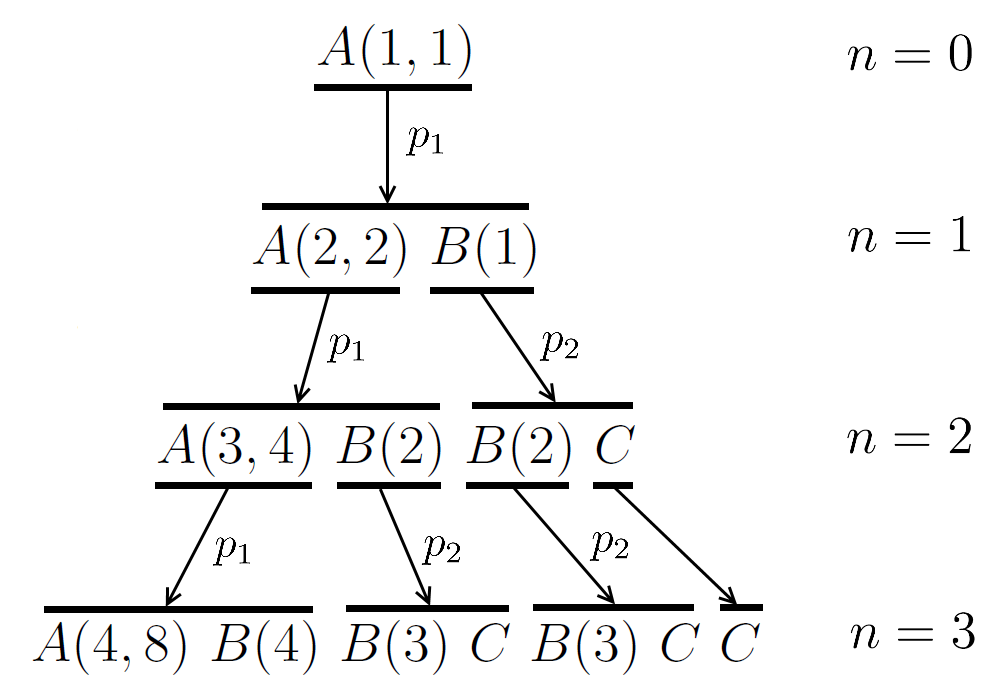
\includegraphics[height=1\textheight]{images/CH2_ParamLSystemBeispiel.png}
\end{center}




\newpage
\slidetitle{}
\subsection{Grafische Interpretation von L-Systemen\\}

\begin{itemize}
	\item Rückgabewerte von L-System-Ableitungen sind Zeichenketten, keine Modelldaten\\
	
	\item Grafische Interpretation von Zeichenketten: Turtle-Interpretation\\
	
	\item Zustand der Turtle ist ein Tupel $(\overrightarrow{p}, \overrightarrow{H})$ mit:
	\begin{description}
		\item[\boldmath$\overrightarrow{p}:$] Position der Turtle\\
		
		\item[\boldmath$\overrightarrow{H}:$] Blickrichtung (Heading) der Turtle
	\end{description}
\end{itemize}






\newpage
\slidetitle{2. L-Systeme -- Grafische Interpretation}

\paragraph{Turtle-Aktionen: \\}

\begin{description}
	\item[\boldmath$F(l):$] Bewegung um $l>0$ in Blickrichtung, Aktualisierung der Position und Zeichnung einer Linie\\
	
	\item[\boldmath$+(d):$]  Drehung um den Winkel $d$ nach links, Aktualisierung der Blickrichtung\\
	
	\item[\boldmath$-(d):$] Drehung um den Winkel $d$ nach rechts, Aktualisierung der Blickrichtung\\
	
	\item[\boldmath$[ \text{ }:$] Ablage des Zustands auf einem Stack\\
	
	\item[\boldmath$\mathbf{]} \text{ }:$] Entnahme des obersten Zustands vom Stack und Aktualisierung des aktuellen Zustands
	
\end{description}




\newpage
\begin{center}
	\begin{minipage}[c]{0.45\textwidth}
		\centering
		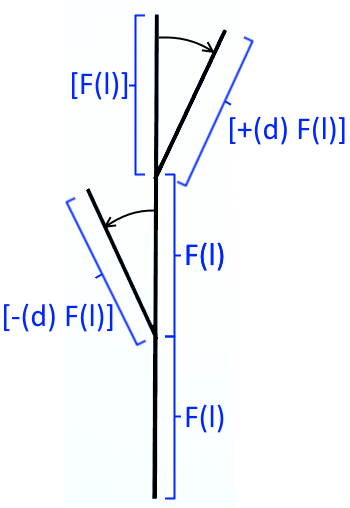
\includegraphics[height=.75\textheight]{images/CH2_Branching2_N1L15D25.png}
		
		$n=1$, $l=240$, $d=25\degree$
	\end{minipage}
	\begin{minipage}[c]{0.45\textwidth}
		\centering
		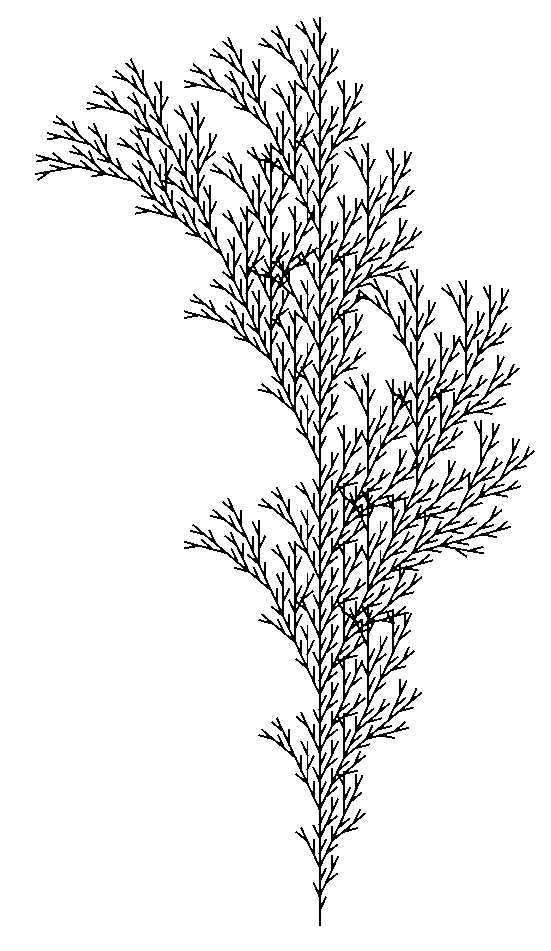
\includegraphics[height=.75\textheight]{images/CH2_Branching2_N5L15D25.png}
		
		$n=5$, $l=15$, $d=25\degree$
	\end{minipage}
	\vspace{0.075\textheight}
	
	$\begin{array}{ll}
	\omega & : F(l) \\
	p_1 & : F(l) \rightarrow F(l)\text{ }[+(d)\text{ }F(l)]\text{ }F(l)\text{ }[-(d)\text{ }F(l)]\text{ }[F(l)]
	\end{array}$
\end{center}



\newpage
\slidetitle{2. L-Systeme -- Anpassungen: 3D Turtle-Interpretation}

\subsection{Anpassungen an Baumstrukturen \\}

\paragraph{Erweiterung der Turtle-Interpretation in den dreidimensionalen Raum}

\begin{itemize}
	\item Zustand der Turtle ist ein Tupel $(\overrightarrow{p}, \boldsymbol{R})$ mit:
	\begin{description}
		\item[\boldmath$\overrightarrow{p}:$] Position der Turtle
		
		\item[\boldmath$\boldsymbol{R}:$] Rotationsmatrix der Turtle\\
	\end{description}
	
	\item Einheitsvektoren $\overrightarrow{H}, \overrightarrow{L}, \overrightarrow{U}$ bilden das lokale Koordinatensystem der Turtle:
	\begin{description}
		\item[\boldmath$\overrightarrow{H}:$] Heading-Vektor
		
		\item[\boldmath$\overrightarrow{L}:$] Left-Vektor
				
		\item[\boldmath$\overrightarrow{U}:$] Up-Vektor
	\end{description}
\end{itemize}





\newpage
\begin{center}
	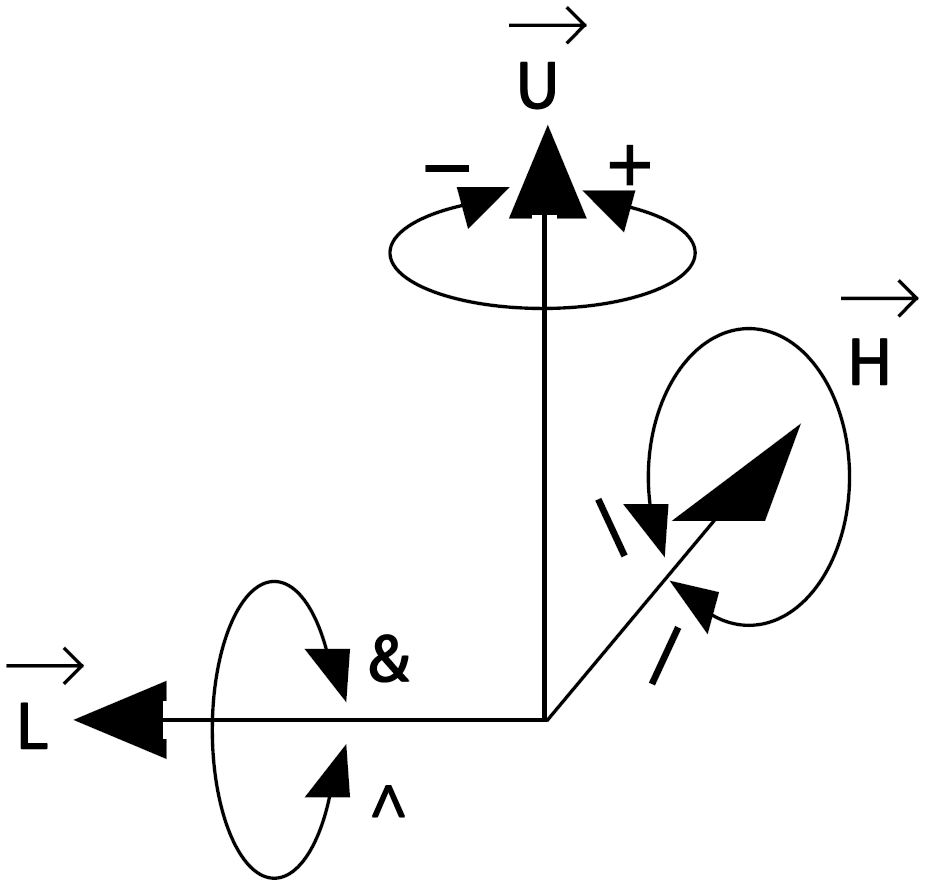
\includegraphics[height=1\textheight]{images/CH2_Turtle3D.png}
	\cite[S.19]{ABOP:04}
\end{center}





\newpage
\begin{center}
	\begin{minipage}[c]{0.6\textwidth}
		\centering
		
\includegraphics[height=.75\textheight]{images/CH2_3DTreeP61B_Angle_18_95.png}
	\end{minipage}
	\begin{minipage}[c]{0.35\textwidth}
			$n=8$, $l=50$, $d=137.5\degree$, 
			
			$a=18.95\degree$, $l_r = 1.3$
	\end{minipage}
\end{center}

\begin{equation}
\begin{array}{llll}
\omega :&  /(45)\text{ }A \\
p_1 :&  A &\rightarrow & F(l)\text{ }[\&(a)F(l)A]\text{ }/(d)\text{ }[\&(a)F(l)A]\text{ }/(d)\text{ }[\&(a)F(l)A] \\
p_2 :& F(l) &\rightarrow & F(l*l_r)
\end{array}
\end{equation}




\newpage
\slidetitle{2. L-Systeme -- Anpassungen: Tropismus}

\paragraph{Einfluss durch Tropismus\\}


\begin{itemize}
	\item Tropismus:Tendenz einer Pflanze in eine bestimmte Richtung zu wachsen\\
	
	\item Einfluss wird als Vektor $\overrightarrow{T} \in \mathbb{R}^3$ angegeben \\
	
	\item Beeinflusst die Bewegung der Turtle in Abhängigkeit des Beugungsfaktors $e \in \mathbb{R}$
\end{itemize}





\newpage
\begin{center}
	
	\begin{minipage}[c]{0.55\textwidth}
		\centering
		
\includegraphics[height=.75\textheight]{images/CH2_3DTreeP61B_Angle_18_95.png}
		\vspace{0.05\textheight}
		
		$\overrightarrow{T} =\begin{pmatrix}
		0 \\ 0 \\ 0
		\end{pmatrix}$, $e = 0$
	\end{minipage}
	\begin{minipage}[c]{0.4\textwidth}
		\centering
		
\includegraphics[height=.75\textheight]{images/CH2_3DTreeP61B_Angle_18_95_Tropism.png}
		\vspace{0.05\textheight}
		
		$\overrightarrow{T} =\begin{pmatrix}
		0 \\ 1 \\ -0.5
		\end{pmatrix}$, $e = 0.27$
	\end{minipage}
\end{center}





\newpage
\slidetitle{2. L-Systeme -- Anpassungen: Graphentheoretischer Baum}

\paragraph{Repräsentation der Turtle-Aktionen als graphentheoretischer Baum\\}

\begin{itemize}
	\item Turtle-Interpretation baut einen graphentheoretischen Baum $G=\langle V,E\rangle$ auf\\
	
	\item Jeder Knotenpunkt $v\in V$ entspricht einem Punkt $\overrightarrow{p}_v \in \mathbb{R}^3$\\
	
	\item Jeder Knotenpunkt besitzt maximal einen Vorgänger und eine endliche Menge von Nachfolgern \\
		
	\item Zustand der Turtle ist ein Tupel $(\overrightarrow{p}, v, \boldsymbol{R})$ mit $v\in V$ \\
	
\end{itemize}




\newpage
\begin{itemize}
	\item Erweiterung der Turtle-Bewegung \boldmath$F(l)$ ausgehend von Zustand $(\overrightarrow{p}, v, \boldsymbol{R})$:
	\begin{itemize}
		\item Bewegung zu Position $\overrightarrow{p_{neu}}$\\
		
		\item Erstellung eines Knotens $v_{neu}$ und einer Kante $(v, v_{neu})$\\
		
		\item Neuer Turtle-Zustand: $(\overrightarrow{p_{neu}}, v_{neu}, \boldsymbol{R})$\\
	\end{itemize}
\end{itemize}



